\documentclass[conference]{IEEEtran}

\usepackage[utf8]{inputenc}
\usepackage[T1]{fontenc}
\usepackage{graphicx}
\usepackage{booktabs}
\usepackage{array}
\usepackage{tabularx}
\usepackage{multirow}
\usepackage{url}
\usepackage{cite}
\usepackage{amsmath}
\usepackage{balance}
\usepackage{xcolor}
\usepackage[hidelinks]{hyperref}

\newcommand{\logminer}{Logminer}
\newcommand{\doiurl}[1]{\href{https://doi.org/#1}{\nolinkurl{doi:#1}}}

\begin{document}

\title{Logminer: Auditable Family-Aware Routing for Heterogeneous Log Anomaly Detection}

\author{
\IEEEauthorblockN{
Andr\'e Olivier Marhegane Bitati\IEEEauthorrefmark{1},
G\'ed\'eon Nkishi Djenga\IEEEauthorrefmark{1},
Jean-Pierre Mugisha Muhire\IEEEauthorrefmark{1}
}
\IEEEauthorblockN{
Josu\'e Lungi Selemani\IEEEauthorrefmark{1},
Christian Kutabuna Kubakisa\IEEEauthorrefmark{1},
Jeff Mugaruka Chihyoka\IEEEauthorrefmark{1},
Witesyavwirwa Vianney Kambale\IEEEauthorrefmark{2},
Kyandoghere Kyamakya\IEEEauthorrefmark{3}
}

\IEEEauthorblockA{\IEEEauthorrefmark{1}
Faculty of Information and Communication Technology, Tshwane University of Technology (TUT), Pretoria, South Africa.
}

\IEEEauthorblockA{\IEEEauthorrefmark{2}
Faculty of Engineering (Polytechnic), Department of Electrical and Computer Engineering, University of Kinshasa, Kinshasa, DR Congo.
}
\IEEEauthorblockA{\IEEEauthorrefmark{3}
Institute for Smart Systems Technologies, University of Klagenfurt, Klagenfurt, Austria.
}

\IEEEauthorblockA{
Corresponding author: Andr\'e Olivier Marhegane Bitati
}

\IEEEauthorblockA{
Emails: aolivier.marhegane@unikin.ac.cd, gedeon.nkishi@unikin.ac.cd, tomsmugisha@unikin.ac.cd
}

\IEEEauthorblockA{
josue.lungi@unikin.ac.cd, christian.kutabuna@unikin.ac.cd, Mugarukachihyoka@gmail.com, kambalevw@tut.ac.za, kyandoghere.kyamakya@aau.at
}
}
\maketitle

\begin{abstract}
Security monitoring environments generate heterogeneous logs whose formats, semantics and statistical distributions differ across operating systems, network flows, SIEM exports and distributed systems. Applying a single monolithic detector to all sources may increase confusion between log families and reduce the interpretability of alerts. This paper presents \logminer, an auditable family-aware routing architecture for anomaly detection in heterogeneous system and network logs.

The prototype decomposes the workflow into specialized cooperating modules for collection, parsing, normalization, family-aware routing, anomaly detection, correlation, dashboard visualization and audit. The contribution is not a new standalone detector, but an auditable specialization layer: events are normalized into a common schema, assigned to a log family with explicit evidence and confidence, processed by a compatible lightweight model, then unified as anomaly candidates before being correlated into analyst-readable incidents.

Experiments cover Windows logs, Wazuh exports, Linux/auth logs, HDFS, BGL, CICIDS2017 and UNSW/CIC-DDoS data. The evaluation includes a controlled common-space ablation and an operational specialization ablation. The results support the feasibility of a local lightweight implementation, while showing that routing should be interpreted as controlled specialization rather than a universal F1 improvement on every dataset.

The prototype is positioned as an analytical complement to mature log management and HIDS/SIEM tools rather than as a replacement for production SOC platforms or large-enterprise SOC infrastructures.
\end{abstract}

\begin{IEEEkeywords}
anomaly detection, log analysis, family-aware routing, multi-model architecture, cybersecurity, lightweight machine learning, SIEM complement, log correlation
\end{IEEEkeywords}

\section{Introduction}
System and network logs are central to security monitoring, incident investigation and operational audit. However, modern infrastructures generate logs from heterogeneous sources: Windows event logs, Linux authentication logs, SIEM/HIDS exports, network-flow datasets, cloud logs and distributed-system traces. These sources differ not only in syntax, but also in event semantics, feature availability, temporal density and class imbalance. This heterogeneity complicates the design of a single anomaly detection pipeline.

Classical intrusion detection and log management research has long emphasized audit trails, deviation from normal behavior and the difficulty of reducing false positives \cite{denning1987intrusion,axelsson2000intrusion,chandola2009anomaly}. More recent machine learning approaches provide promising results, but remain sensitive to dataset shift, closed-world assumptions, class imbalance and operational interpretability \cite{sommer2010outside,buczak2016survey,khraisat2019survey}. In practice, operational tools such as fail2ban, OSSEC, Wazuh or ELK-like stacks provide valuable collection, rule-based detection, indexing and visualization, but they do not by themselves solve the problem of controlled model specialization across heterogeneous log families.

This paper introduces \logminer, a lightweight prototype designed to evaluate a family-aware multi-model strategy for heterogeneous log anomaly detection. The term agent is used here in a software architectural sense: \logminer{} is composed of specialized cooperating modules with distinct functional roles, message exchange and workflow coordination. The prototype does not claim to implement fully autonomous cognitive agents, FIPA-style negotiation, reinforcement-learning cooperation or LLM-agent autonomy. It includes a bounded supervisor agent that performs a perception-state-decision-action cycle for local workflow adaptation, but this supervisor is treated as an implementation control layer rather than as the main scientific contribution.

The central research question is: when and why can auditable family-aware routing improve heterogeneous log anomaly detection compared with monolithic alternatives? The answer is not expected to be universal. Routing is evaluated as a mechanism that enables compatible feature spaces, explicit fallback behavior, interpretable routing reasons and family-specific operational policies.

The contribution of this paper is fourfold:
\begin{enumerate}
    \item An auditable family-aware software-agent architecture for log analysis, including collector, parser, normalizer, router, detector, correlator, dashboard, audit and bounded supervisor roles.
    \item A formal routing and fallback mechanism in which normalized logs are assigned to a log family through explicit evidence, confidence scoring and route explanations before being processed by a compatible detector.
    \item A multi-source evaluation covering system logs, SIEM exports and network datasets, including controlled and operational ablations, false positives, routing audit traces, bounded local workflow latency and operational limits.
    \item A cautious empirical positioning showing that family-aware routing is controlled specialization rather than a guaranteed F1 improvement on every dataset.
\end{enumerate}

The paper deliberately uses cautious claims. Non-supervised outputs are treated as anomaly candidates, not confirmed intrusions. The validated distribution is mainly logical and modular, while large-scale multi-machine distribution remains future work. The source code of the prototype is available at \url{https://github.com/andybitati/Memoire}; large raw datasets and local operational exports are excluded from the repository when size, licensing or privacy constraints apply. The remainder of the paper is organized as follows: Section II reviews related work, Sections III and IV present the methodology and routing mechanism, Section V details the implementation, Section VI describes the experimental setup, Section VII reports and discusses the results, Section VIII states the operational positioning and validity limits, and Section IX concludes the paper.

\section{Related Work}
\subsection{Anomaly Detection and Intrusion Detection}
Denning's intrusion detection model introduced the idea of detecting deviations from expected user and system behavior through audit records \cite{denning1987intrusion}. Axelsson later structured IDS concepts and taxonomies, while Chandola et al. provided a broader survey of anomaly detection methods across point, contextual and collective anomalies \cite{axelsson2000intrusion,chandola2009anomaly}. These foundations are directly relevant to log anomaly detection, where isolated rare events and correlated sequences may indicate abnormal behavior.

Machine learning has been widely investigated for cyber intrusion detection. Buczak and Guven review data mining and machine learning methods for cybersecurity, while Khraisat et al. discuss IDS datasets, challenges and evaluation issues \cite{buczak2016survey,khraisat2019survey}. Sommer and Paxson warn against overinterpreting machine learning results in intrusion detection, especially when training and testing assumptions do not reflect operational environments \cite{sommer2010outside}. This warning motivates the cautious positioning adopted in this work.

\subsection{Log Parsing and Log-Based Detection}
Before machine learning can be applied, raw logs must be parsed and transformed into usable representations. Template-based approaches such as Drain organize log messages into event templates and enable downstream sequence or statistical modeling \cite{he2016drain}. Public benchmark resources such as LogHub have also helped structure evaluation around reusable system-log datasets and parsing tasks \cite{zhu2023loghub}. DeepLog and related approaches model log sequences with deep learning to detect deviations from normal execution patterns \cite{du2017deeplog}. LogAnomaly extends this line by combining sequential and quantitative anomaly signals, LogRobust addresses unstable log events with semantic vectors and attention-based sequence modeling, and LogBERT uses self-supervised Transformer-style modeling for log sequences \cite{meng2019loganomaly,zhang2019logrobust,guo2021logbert}. These methods are powerful for homogeneous sequential logs, but applying the same sequence model indiscriminately to all enterprise sources is technically and economically difficult: Windows events, Linux authentication lines, SIEM exports, cloud JSON records and network flows do not share a single event grammar, sequence length, sampling rhythm or feature contract. A monolithic deep sequence model would therefore require costly global preprocessing, padding or template alignment, and would still risk learning dominant families while weakening minority sources. \logminer{} takes a different route: it first normalizes enough information for audit and routing, then selects a compatible family-specific branch. Lightweight parsing is used in this first version, while template-based parsing is retained as a natural extension for Linux, HDFS and BGL-style logs.

\subsection{Agent-Based Security Monitoring}
Agent-based security monitoring has historical roots in distributed intrusion detection. AAFID proposed an architecture using autonomous agents to collect and analyze host-level events before aggregation \cite{balasubramaniyan1998aafid}. \logminer{} follows this lineage in a more modest way: agents are software modules and services with clear responsibilities and exchange contracts. The goal is not full cognitive autonomy, but controlled specialization, modular replacement and future deployability.

\subsection{Routing, Expert Selection and Network Anomaly Detection}
The proposed router is related in spirit to mixture-of-experts systems, where a gating mechanism assigns inputs to specialized experts \cite{jacobs1991moe}. However, \logminer{} deliberately avoids presenting the current router as a learned probabilistic gate. Its routing rules are auditable policy evidence, designed to expose why a family and detector were selected and when fallback was triggered. This makes the mechanism closer to operational model selection than to end-to-end expert learning.

For network-flow anomaly detection, lightweight tabular models and online neural approaches both exist. Kitsune, for example, uses an ensemble of autoencoders for online network intrusion detection \cite{mirsky2018kitsune}. \logminer{} does not claim to replace specialized NIDS algorithms; its contribution is the routing layer that can decide when network-flow records should be processed by a network-compatible detector rather than by a system-log branch.

\section{Methodology}
\subsection{Architectural Scope}
The proposed architecture follows a log processing chain from raw sources to analyst-readable incidents. Fig.~\ref{fig:architecture} summarizes the logical workflow. Each agent has a restricted responsibility: the collector retrieves or receives raw logs; the parser detects formats and extracts fields; the normalizer maps extracted fields to a common schema; the router assigns events to a log family; the detector applies a family-specialized model; the correlator groups anomaly candidates into incidents; and the dashboard exposes results for human validation and audit.

\begin{figure*}[t]
    \centering
    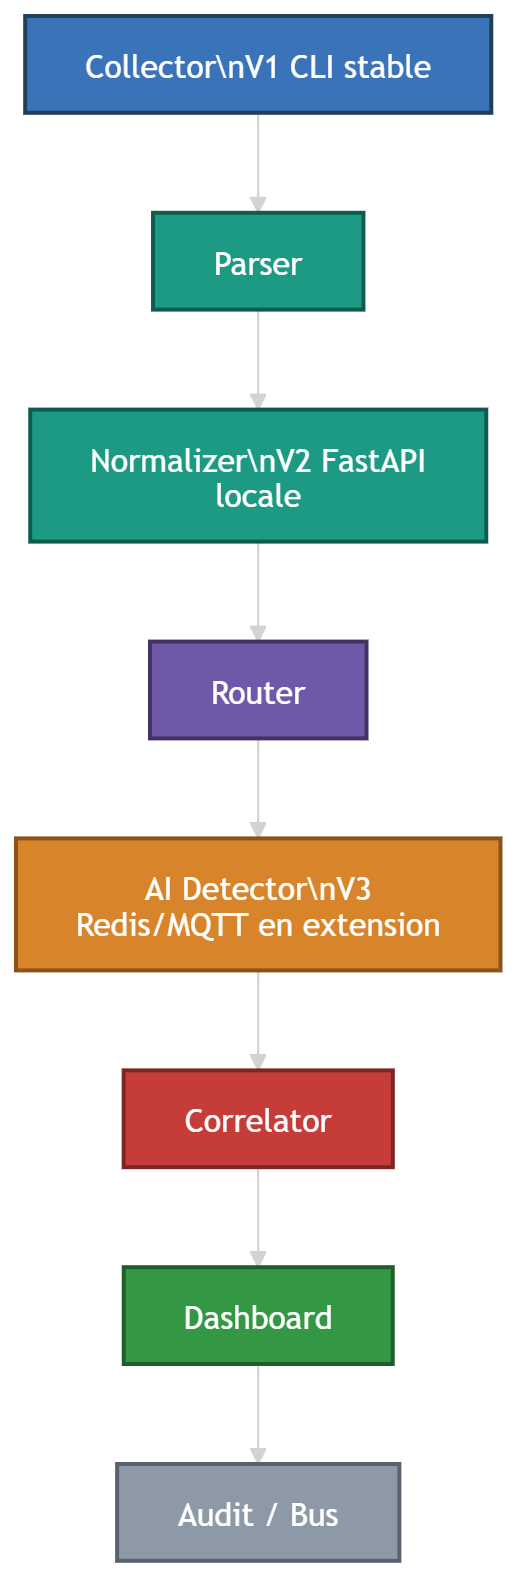
\includegraphics[height=0.6\textheight,keepaspectratio]{figures/fig_architecture_logminer_readable.png}
    \caption{Logical architecture of \logminer. The contribution is the controlled path from heterogeneous inputs to family-aware model selection and analyst-readable incident candidates, not a new standalone detector.}
    \label{fig:architecture}
\end{figure*}

The distribution validated in this work is primarily logical and modular. The service-level implementation is partially supported through FastAPI endpoints, a local JSONL bus and an optional Redis Streams evolution. Redis Streams supports service traces and a queued workflow mode in which API requests can enqueue jobs consumed by external workers through consumer groups. In this first article, this is reported only as an implementation boundary that prevents the architecture from being tied to synchronous calls; no Redis throughput, worker-scaling or fault-recovery result is used as core evidence. Large-scale multi-machine deployment and operational scalability evaluation are reserved for the companion operational article.

\subsection{Agent Roles and Interaction}
Table~\ref{tab:agents} summarizes the main agents. This decomposition is important because it prevents the detector from becoming an opaque monolithic block. It also allows future replacement of one agent without redesigning the entire pipeline.

\begin{table}[t]
\caption{Specialized agents in the \logminer{} architecture}
\label{tab:agents}
\centering
\scriptsize
\begin{tabularx}{\linewidth}{p{1.5cm}X X}
\toprule
\textbf{Agent} & \textbf{Role} & \textbf{Output} \\
\midrule
Collector & Retrieves local or exported logs from Windows, Linux, SIEM or dataset folders & Raw files and manifests \\
Parser & Detects format and extracts timestamp, host, event, severity, source and message fields & Structured events \\
Normalizer & Maps heterogeneous fields to a common event schema & Normalized records \\
Router & Identifies the family of each log batch or event stream & Model selection decision \\
Detector & Applies a lightweight supervised or non-supervised model specialized by family & Anomaly candidates \\
Correlator & Groups anomalies by time, source, host, severity or context & Interpretable incidents \\
Dashboard/Audit & Displays events, anomalies, incidents and analyst decisions & Visual analysis and traceability \\
Supervisor & Observes sources/resources and adapts workflow parameters & Policy-based bounded workflow control \\
\bottomrule
\end{tabularx}
\end{table}

Communication is implemented through file-based artifacts, JSONL messages, FastAPI endpoints and optional Redis Streams evolution. Coordination is handled by an orchestrated workflow, including discovered-source execution and route-based processing.

\subsection{Normalized Event Contract}
The common schema contains fields such as timestamp, severity, event identifier, source, host, user, source and destination IP, ports, category, subcategory and message. This common representation does not erase family-specific information; it provides the minimal interface required for model routing, scoring, correlation and visualization. The design follows log management principles in which normalization and retention of raw context are both necessary for auditability \cite{nist80092,rfc5424}.

\section{Family-Aware Routing Mechanism}
\subsection{Motivation}
The central hypothesis of this work is that log families exhibit sufficiently different structures and distributions to justify specialized detection models. Windows event logs, Linux/auth logs, Wazuh alerts, HDFS traces, BGL HPC logs and network-flow datasets do not expose the same fields, semantics or anomaly patterns. A single global model may therefore learn dominant distributions from one family and behave poorly on another.

\logminer{} addresses this issue through family-aware routing. After normalization, each batch or stream is associated with a log family. The router selects a model compatible with that family. The detector then produces anomaly candidates in a unified output format, allowing downstream correlation and dashboard analysis.

\begin{figure}[t]
    \centering
    
\includegraphics[width=\linewidth]{figures/fig_model_portfolio_scale.pdf}
    \caption{Model portfolio used by \logminer{} across Windows, Wazuh, Linux/auth, network, HDFS, BGL and fallback families. Each artifact is selected according to routing confidence and family compatibility.}
    \label{fig:models}
\end{figure}

\subsection{Scientific Claim}
The novelty is not the isolated use of parsing, machine learning or a dashboard. The novelty is an auditable specialization layer: heterogeneous logs are normalized, routed according to family, scored by compatible lightweight models and correlated into incidents while preserving the route evidence that led to model selection. This strategy aims to improve robustness and analyst usability in the presence of heterogeneous formats and distributions; this hypothesis must be evaluated experimentally against monolithic baselines. The claim is therefore architectural and experimental rather than algorithmically theoretical. A negative or neutral result on one dataset does not invalidate the claim if the architecture still exposes route reasons, fallback behavior and feature/model compatibility boundaries.

\subsection{Router Formalization}
Let $x$ be a normalized event batch, $\mathcal{F}$ the set of supported log families, and $M_f$ the detector associated with family $f \in \mathcal{F}$. The router computes a compatibility score:
\begin{equation}
    S(f,x) = w_n N(f,x) + w_c C(f,x) + w_m M(f,x),
\end{equation}
where $N(f,x)$ measures filename or source-name evidence, $C(f,x)$ measures the presence of expected normalized or native columns, and $M(f,x)$ measures marker tokens observed in sampled values. The selected family is:
\begin{equation}
    f^{*} = \arg\max_{f \in \mathcal{F}} S(f,x),
\end{equation}
with confidence:
\begin{equation}
    \gamma(x) = \frac{S(f^{*},x)}{\sum_{f \in \mathcal{F}} S(f,x) + \epsilon}.
\end{equation}
If $\gamma(x) < \tau$ or if mandatory evidence is missing, the router selects the fallback detector. The detector output is then represented as a unified anomaly candidate:
\begin{equation}
    a = \langle t, h, f^{*}, m, y, q, r \rangle,
\end{equation}
where $t$ is the timestamp, $h$ the host or source, $m$ the selected model, $y$ the predicted candidate label, $q$ the anomaly score or confidence, and $r$ the routing reason. This formalization makes the routing decision auditable without claiming a learned routing policy.

The weights $w_n$, $w_c$ and $w_m$ are fixed policy parameters in the current prototype. They are set empirically to favor high-confidence structural evidence before weaker lexical cues: explicit family columns and dataset-specific fields receive the strongest contribution, marker tokens provide supporting evidence, and source-name evidence is used mainly as a tie-breaker or early hint. The implementation also uses priority ordering and fallback thresholds to avoid brittle decisions when evidence is sparse. Table~\ref{tab:router_weights} reports the exact additive constants used in the current prototype. In practice, routing decisions are not expected to be highly sensitive to small perturbations such as changing the generic column weight from $+8$ to $+10$, because most supported families are separated by multiple simultaneous signals and by fallback priority rules rather than by a single marginal feature.

The different magnitudes in Table~\ref{tab:router_weights} should be read as rule-specific additive evidence rather than as globally comparable learned coefficients. Heavy constants are attached to highly discriminative markers or to fallback-only conditions, and they are applied only when the corresponding evidence is present for the candidate family. A sparse family such as Linux/auth is therefore not penalized merely because another family has a larger possible maximum score; unsupported or absent descriptors do not contribute to competing families. The confidence $\gamma(x)$ is used as an audit and fallback signal together with mandatory evidence checks, not as the only routing criterion. A softmax or MinMax normalization could make scores numerically comparable, but it could also inflate weak noisy evidence when all families have low support. For this first prototype, explicit evidence thresholds and fallback routing were preferred for interpretability; calibrated score normalization remains future work.

As a limited local sensitivity check, the five distinct sources used in the SupervisorAgent campaign were replayed after normalization while applying a uniform $\pm 10\%$ perturbation to the additive evidence constants. The selected families remained unchanged: CEF, CloudTrail, Apache and corrupted inputs were routed to fallback, while Linux/auth was routed to the Linux branch. This check does not replace a complete factorial sensitivity analysis, but it indicates that the reported supervisor routes do not depend on a single marginal weight change.

\begin{table}[t]
\caption{Local routing sensitivity on SupervisorAgent sources}
\label{tab:router_sensitivity}
\centering
\scriptsize
\begin{tabularx}{\linewidth}{p{2.4cm}p{1.5cm}p{1.5cm}X}
\toprule
\textbf{Source type} & \textbf{Expected} & \textbf{$\pm10\%$ route} & \textbf{Interpretation} \\
\midrule
CEF/LEEF & fallback & stable & Unsupported SIEM-like format is preserved without claiming a specialized detector \\
CloudTrail & fallback & stable & Cloud JSON records are retained as fallback in this article \\
Apache access & fallback & stable & Web logs are not forced into the network-flow detector after normalization \\
Linux/auth syslog & linux & stable & Syslog evidence dominates generic Windows-like normalized columns \\
Corrupted input & fallback & stable & Unknown/corrupted markers trigger graceful degradation \\
\bottomrule
\end{tabularx}
\end{table}

Because the router is a distinct architectural component, detector-level F1 is not sufficient to evaluate it. A complete router evaluation should also report route accuracy when family labels are known, fallback precision on unsupported sources, low-confidence rate, route stability under perturbed weights, and misroute severity when an event is sent to an incompatible detector. The current paper reports routing behavior through ablations, fallback tests and audit traces, but these router-specific metrics remain a target for a stricter artifact evaluation.

\begin{table*}[t]
\caption{Numerical routing policy constants used in the prototype}
\label{tab:router_weights}
\centering
\scriptsize
\begin{tabularx}{\textwidth}{p{2.7cm}r p{4.7cm}X}
\toprule
\textbf{Evidence} & \textbf{Weight} & \textbf{Activation condition} & \textbf{Purpose in current router} \\
\midrule
Matched family column & $+8$ each & Column name belongs to the candidate family's allow-list & Low-cost structural evidence; several columns must usually accumulate before a family dominates \\
Generic family marker & $+35$ & Family token appears in sampled values or dataset/subtype fields & Supporting lexical evidence; never used alone as a production claim \\
Network feature bundle & $+12$ per hit & Active source/destination IPs, ports, protocol, packet/byte counters, attack labels or visible IP values & Separates tabular network-flow files from operating-system event logs \\
CICIDS feature bundle & $+80 + 8h$ & At least five CICIDS columns are present; $h$ is the number of matched CICIDS columns & Routes MachineLearningCVE-style flows to the CICIDS-compatible model \\
Windows feature bundle & $+10h$ & Microsoft provider tokens, numeric EventID density, EVTX source markers, or Windows host/user/session fields & Routes normalized Windows event logs without relying only on filenames \\
HDFS/BGL feature bundle & $+12h$ & HDFS block/NameNode/DataNode markers or BGL/RAS/BlueGene markers; $h$ is the matched feature count & Detects sequential system-log families while exposing their current detector limits \\
Wazuh/SIEM bundle & $+90+8h$ or $+120+12h$ & Wazuh raw columns or normalized Wazuh fields are present; subtype and OSSEC/Wazuh markers add supporting evidence & Prevents SIEM exports from being treated as ordinary Linux or Windows logs \\
Linux/auth bundle & $+70+8h$ & At least three authentication columns plus source IP and port are present & Keeps authentication datasets out of the generic network branch despite shared IP/port fields \\
Filename hint & $+45$ & Path contains known CICIDS/MachineLearningCVE or Linux/auth identifiers & Tie-breaker for curated benchmark files, not a substitute for structural evidence \\
Dense network profile & $+20$ & At least 15 numeric columns and at least 25 total columns & Weak transverse signal for network-like tabular data \\
Known unsupported subtype & $+140$ fallback & Apache, CEF/LEEF, CloudTrail or all-unknown dataset/subtype markers & Forces graceful fallback when no specialized model is claimed in this article \\
Corrupted input marker & $+120$ fallback & Path or sampled text contains corrupt, incomplete or broken markers & Preserves malformed inputs without forcing them into a specialized detector \\
Syslog subtype & $+140$ linux, $-40$ windows & Normalized subtype contains syslog & Prevents syslog batches from being routed to Windows when fields overlap \\
\bottomrule
\end{tabularx}
\end{table*}

\subsection{Ablation Protocol}
To make the claim testable, the experimental protocol includes an ablation study. Table~\ref{tab:ablation} defines the comparisons. Two levels are reported. First, a controlled common-space ablation forces both the global model and the family-aware models to use the same minimal feature representation. Second, an operational ablation compares the same global common-feature baseline with the full specialized configurations, where each family can use its native feature space and trained detector. A complete factorial isolation of routing, features and model family is identified as future work; the present evaluation separates a constrained routing effect from the complete specialization package.

A stricter future factorial design should independently vary the router type, feature representation, detector family, correlation policy and fallback policy. Such a design would separate the effect of selecting the right family from the effect of using richer native features or stronger downstream models.

\begin{table}[t]
\caption{Ablation protocol used to evaluate family-aware specialization}
\label{tab:ablation}
\centering
\scriptsize
\begin{tabularx}{\linewidth}{p{2.4cm}X}
\toprule
\textbf{Configuration} & \textbf{Purpose} \\
\midrule
Global common model & Main baseline: one detector applied to all families using a minimal shared feature space \\
Family-aware common models & Controlled test: family selection and per-family detectors under the same minimal shared features \\
Family-aware native models & Operational test: routing plus family-compatible native features and specialized detectors \\
Without correlation & Measures detector-level candidate production before incident grouping \\
With correlation & Measures the complete pipeline from anomaly candidate to analyst-readable incident \\
Factorial routing/features/models & Future Work: planned extension to isolate the independent causal effect of each component \\
\bottomrule
\end{tabularx}
\end{table}

Table~\ref{tab:claim_boundaries} maps the main hypotheses to the level of evidence available in this paper. This table is included to make the contribution falsifiable and to separate demonstrated behavior from future work.

\begin{table}[t]
\caption{Hypotheses and evidence boundaries}
\label{tab:claim_boundaries}
\centering
\scriptsize
\begin{tabularx}{\linewidth}{p{1.7cm}X X}
\toprule
\textbf{Hypothesis} & \textbf{Expected behavior} & \textbf{Evidence boundary} \\
\midrule
H1 & A monolithic common model can remain competitive when all families use the same minimal features & Confirmed by the controlled ablation; routing alone is not claimed as universally superior \\
H2 & Family-aware routing helps when it enables native feature spaces and compatible detectors & Supported for Linux/auth and UNSW in the operational ablation; CICIDS is already near saturation \\
H3 & Sequential system logs require sequence-aware branches & Supported as a limitation by HDFS false positives; Drain-like and temporal detectors remain future work \\
H4 & Fallback routing prevents unknown or corrupted inputs from breaking the workflow & Supported as graceful degradation; fallback outputs are not confirmed intrusions \\
H5 & The routing layer is feasible on a local workstation or gateway & Supported by local latency and routing-overhead results; SOC-scale throughput is not claimed \\
\bottomrule
\end{tabularx}
\end{table}

\subsection{Fallback Routing}
The fallback model is selected when the router cannot assign a source to a known family with sufficient evidence from file type, column names, marker tokens or sampled values. It is also selected for records explicitly normalized as unknown or marked as corrupted/incomplete. It is not intended to maximize detection performance. Its role is graceful degradation: unknown formats still produce low-confidence anomaly candidates instead of silently breaking the pipeline. Fallback outputs therefore require correlation or analyst validation before interpretation.

\begin{table}[t]
\caption{Fallback behavior on corrupted input}
\label{tab:fallback}
\centering
\scriptsize
\begin{tabular}{l r l r r r}
\toprule
\textbf{Input} & \textbf{Rows} & \textbf{Route} & \textbf{Score} & \textbf{Cand.} & \textbf{Inc.} \\
\midrule
corrupt\_incomplete.log & 2 & fallback & 141 & 0 & 0 \\
\bottomrule
\end{tabular}
\end{table}

\section{Implementation}
The prototype is implemented in Python with a modular source tree. The stable version uses command-line execution, CSV artifacts and local folders. The service-oriented version exposes core workflow actions through FastAPI, including source discovery, detection and correlation. A local JSONL bus supports message-oriented traces, while Redis Streams is implemented as an optional extension for service-level experiments, queued workflow execution and worker-based processing. The present article does not evaluate this queue as a scalability result; it only documents that the architecture has a non-blocking evolution path.

The current local buffering strategy is intentionally simple. Collectors and parsers persist raw files, manifests, normalized records and bus messages as local file artifacts before detection. The detector then processes bounded samples or prepared batches rather than keeping an unbounded in-memory queue. To reduce API blocking, the Redis extension adds a persistent job stream, consumer-group reading, acknowledgement of completed jobs and a standalone worker script. These mechanisms are mentioned here to clarify deployability, not to claim a measured scalability contribution. If detection lags behind collection, the backlog remains visible in files, JSONL traces and Redis pending-job summaries. However, the prototype does not yet implement production-grade admission control, adaptive back-pressure, retry policies, dead-letter handling or priority scheduling. This design is acceptable for a local analytical prototype or intermediate gateway, but it is not sufficient for large-enterprise ingestion under bursty or adversarial traffic; Kafka, MQTT, Redis Streams with fully tested worker policies, or an equivalent broker would be needed for durable asynchronous scaling. Detailed queue, worker and resource behavior is outside this article and belongs to the operational evaluation.

The detector portfolio includes supervised Random Forest models for labeled families such as Linux/auth, CICIDS2017 and UNSW/CIC-DDoS, as well as non-supervised Isolation Forest or ensemble-style detectors for sources where labels are incomplete or absent. Non-supervised outputs are explicitly called anomaly candidates.

A web dashboard supports exploration of anomalies, incidents, counters, filters, timeline-style views and analyst decisions. This dashboard is an exploitation layer: it does not prove the anomaly by itself, but helps analysts validate, reject or reinterpret candidate incidents.

\subsection{Correlation Logic}
The correlator is intentionally explainable rather than opaque. It groups anomaly candidates by a configurable temporal window, host, user, source, category, subcategory, protocol and destination port. Incident priority combines event volume, maximum severity, diversity of event identifiers, security category weight and anomaly-score depth. For a candidate set $A$, the correlator emits an incident $I$ when candidates share a context key and fall within the window $\Delta t$. The default $\Delta t=15$ minutes was chosen as a conservative analyst-triage window for local workstation experiments; the SupervisorAgent can raise it to 20 minutes when fallback routes dominate and to 30 minutes for sequential system-log families such as HDFS/BGL. These values are policy parameters, not optimized thresholds. The priority score is a weighted combination of candidate count, severity, source diversity and anomaly-score depth. This correlation step improves analyst readability, but it is treated as a pipeline component rather than as the main algorithmic contribution of the paper. The present evaluation reports the resulting incidents and timing overhead; it does not prove that every merged incident is analytically correct. A dedicated correlation-quality evaluation with analyst labels, window-size sensitivity and incorrect-merge analysis remains future work.

\subsection{Policy-Based Workflow Orchestration and Control}
The current implementation uses software agents with specialized roles, explicit message exchange and workflow coordination. A bounded SupervisorAgent was added only to coordinate local workflow execution and to preserve route-level audit evidence. It observes available log candidates, chooses a source and workflow parameters, launches parsing, routing, detection and correlation, then records each decision in audit and bus traces. The current decisions are policy-based and explainable rather than learned; therefore, the supervisor is treated here as an implementation control layer, not as the main adaptive-AI contribution. Table~\ref{tab:supervisor} summarizes a controlled 30-cycle trace used to verify that routing decisions remain replayable.

\begin{table}[t]
\caption{Policy-based SupervisorAgent campaign}
\label{tab:supervisor}
\centering
\scriptsize
\begin{tabular}{l l}
\toprule
\textbf{Indicator} & \textbf{Value} \\
\midrule
Completed cycles & 30/30 \\
Distinct selected sources & 5 \\
Routed families & fallback, linux \\
Mean cycle duration & 9.3047 s \\
Maximum cycle duration & 13.0508 s \\
Window range & 15--20 min \\
Sample range & 300--1000 rows \\
Audit trace recorded & yes \\
\bottomrule
\end{tabular}
\end{table}

In this controlled campaign, unsupported web/SIEM/cloud formats were routed to fallback, syslog-like records were routed to the Linux branch, and every decision recorded the selected source, family, sample size, window size and status. The correlation window remained bounded at 15--20 minutes and no sampling oscillation was observed. Broader stress behavior, source quarantine, degradation budgets and long-running resource control are deliberately left outside the main contribution of this article and are better suited to a separate operational evaluation.

For the five distinct SupervisorAgent sources, the route-level confusion matrix is reported in Table~\ref{tab:router_confusion}. The matrix evaluates the routing decision after parsing/normalization, which is the actual input stage used by the supervisor workflow. It should not be confused with detector-level intrusion classification: unsupported CEF/LEEF, CloudTrail, Apache and corrupted inputs are expected to fall back, whereas Linux/auth syslog is expected to use the Linux branch. Under this protocol, the route accuracy is $5/5$ at distinct-source level and $30/30$ across the repeated supervisor cycles.

\begin{table}[t]
\caption{Route-level confusion matrix for SupervisorAgent sources}
\label{tab:router_confusion}
\centering
\scriptsize
\begin{tabular}{lcc}
\toprule
\textbf{Expected route} & \textbf{Predicted fallback} & \textbf{Predicted linux} \\
\midrule
fallback & 4 & 0 \\
linux & 0 & 1 \\
\bottomrule
\end{tabular}
\end{table}

\section{Experimental Setup}
Table~\ref{tab:datasets} lists the families used in the initial evaluation. The selection mixes local logs, SIEM-style exports, public system logs and public network datasets.

\begin{table*}[t]
\caption{Datasets and scenarios used in the initial evaluation}
\label{tab:datasets}
\centering
\scriptsize
\begin{tabularx}{\textwidth}{p{2.2cm}p{3.1cm}p{2.8cm}X}
\toprule
\textbf{Category} & \textbf{Source} & \textbf{Nature} & \textbf{Objective} \\
\midrule
Local real & Windows Event/Application/System/Security & Windows system logs & Test EVTX/XML collection, parsing and local candidate detection \\
Real/SIEM & Wazuh exports & SIEM/HIDS events and alerts & Test non-supervised detection on operational security signals \\
Real tabular & Linux/auth & Labeled authentication logs & Supervised evaluation and false positive analysis \\
Public system & HDFS & Distributed-system logs with labels & Validate detectors on sequential system logs \\
Public system & BGL & BlueGene/L logs with labels & Validate detectors on HPC logs \\
Public network & CICIDS2017 & Labeled network flows & Supervised detection of known attack classes \\
Public network & UNSW/CIC-DDoS & Network/DDoS flows & Chunk-based 80/20 evaluation \\
Robustness & Apache, CEF/LEEF, CloudTrail, Linux auth, incomplete log & Multi-format and corrupted input & Test parser tolerance and preservation of unknown records \\
\bottomrule
\end{tabularx}
\end{table*}

\subsection{Evaluation Protocol and Experimental Rigor}
The evaluation follows a validation-based protocol adapted to the heterogeneous nature of the sources. For labeled supervised datasets, metrics are reported on held-out test partitions or predefined evaluation splits, using F1-score and false positive rates to capture both detection quality and analyst workload. For unlabeled operational exports, such as Wazuh or local Windows logs, outputs are explicitly interpreted as anomaly candidates and correlated incidents rather than confirmed attacks. Workflow latency is reported only to verify that the routing layer is feasible in a local prototype; detailed resource, stress and scalability behavior is outside the core scope of this first article.

The routing ablation is split into two complementary views. The controlled common-space comparison constrains all families to the same minimal representation, whereas the operational comparison evaluates the full specialization package composed of family identification, native feature compatibility and specialized model selection. This protocol is designed to reduce overclaiming: the controlled ablation tests whether routing alone dominates under shared features, while the operational ablation tests whether routing enables compatible feature spaces and models. All results should therefore be read as evidence for a lightweight family-aware analytical architecture, not as a universal benchmark victory over all monolithic or sequence-aware detectors.

The experimental artifacts were organized to support manuscript-level traceability: routed outputs, anomaly candidates, incidents, timing profiles, resource snapshots, figures and LaTeX tables are preserved as local files before being summarized in the paper. The GitHub repository mentioned in the introduction includes the executable source tree together with the development requirements, a pinned container requirements file, a Dockerfile for the FastAPI runtime, and Redis/MQTT Docker Compose descriptors. Large datasets, local exports and trained model binaries may remain external when size, licensing or privacy constraints apply.

\section{Results and Discussion}
\subsection{Detection Results}
Table~\ref{tab:results} summarizes the principal results available in the current prototype. The supervised Random Forest models obtain strong F1 scores on CICIDS2017 and UNSW/CIC-DDoS, and a lower but still usable score on Linux/auth. HDFS remains more difficult with the current lightweight features, whereas BGL obtains high validation scores.

\begin{table*}[t]
\caption{Principal detection results available in the prototype}
\label{tab:results}
\centering
\scriptsize
\begin{tabularx}{\textwidth}{p{2.0cm}p{3.4cm}p{3.2cm}X}
\toprule
\textbf{Family} & \textbf{Dataset} & \textbf{Model} & \textbf{Main result} \\
\midrule
Windows & Security/Application/System & Isolation Forest & Anomaly candidates and correlated incidents \\
Wazuh & January/October/December exports & Isolation Forest & 122,563 events and 3,676 anomaly candidates \\
Linux/auth & Authentication logs & Random Forest & F1 = 0.916602 \\
CICIDS & CICIDS2017 MachineLearningCVE & Random Forest & F1 = 0.997163 \\
UNSW/CIC-DDoS & UNSW-NB15/CIC-DDoS network data & Random Forest & F1 = 0.999965 \\
HDFS & Distributed-system logs & Ensemble / Isolation Forest & Best selection around F1 = 0.599333 \\
BGL & BlueGene/L HPC logs & Ensemble / Autoencoder / Isolation Forest & Best selection around F1 = 0.994333 \\
\bottomrule
\end{tabularx}
\end{table*}

\begin{figure}[t]
    \centering
    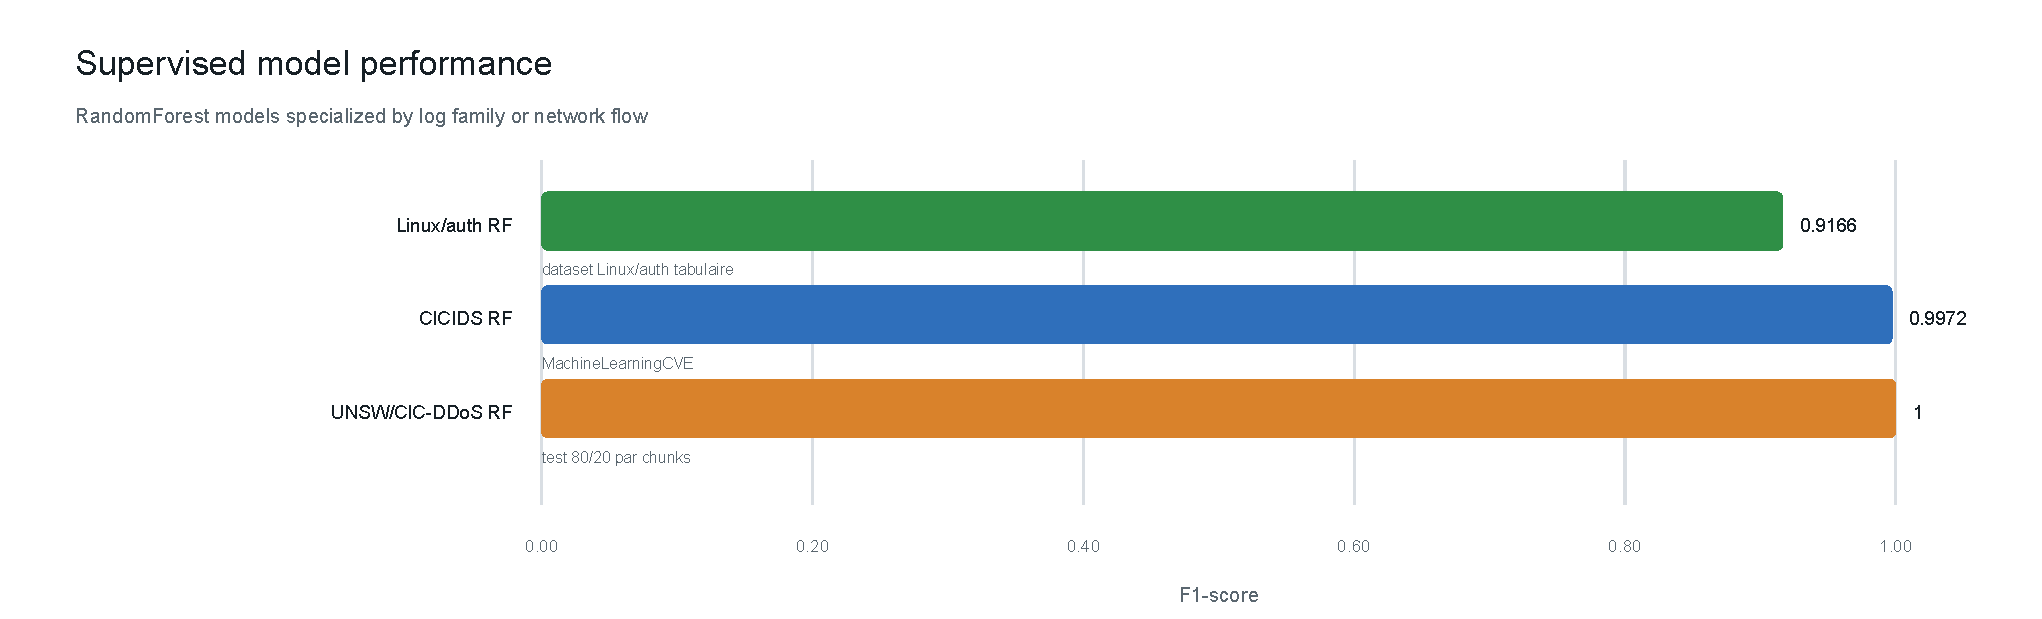
\includegraphics[width=\linewidth]{figures/fig_supervised_models_f1.pdf}
    \caption{F1-score of supervised Random Forest models on Linux/auth, CICIDS2017 and UNSW/CIC-DDoS families.}
    \label{fig:f1}
\end{figure}

These results should not be interpreted as universal superiority. They show that the prototype can integrate several families and that family-specific models are operationally feasible. The routing effect is therefore isolated through the ablations below.

\subsection{Routing Audit Evidence}
Since the paper now centers on auditable routing, the evaluation must expose what is actually audited. In the current prototype, each routed execution records the selected family, route reason, route score or confidence signal, selected model branch and downstream candidate/incidence counts. Table~\ref{tab:routing_audit} summarizes the evidence that is already available from the current artifacts. These results do not constitute a complete route-accuracy benchmark, but they show that route decisions are inspectable rather than hidden inside the detector.

\begin{table}[t]
\caption{Routing audit evidence available in the prototype}
\label{tab:routing_audit}
\centering
\scriptsize
\begin{tabularx}{\linewidth}{p{2.0cm}X X}
\toprule
\textbf{Evidence} & \textbf{Observed behavior} & \textbf{Interpretation} \\
\midrule
Corrupted input & 2 rows preserved, routed to fallback with route score 141 & Unknown records are not silently discarded or forced into a specialized family \\
Supervisor trace & 30/30 cycles recorded selected source, routed family, sample size, window size and status & Routing decisions are replayable through audit and bus traces \\
Unsupported formats & CEF, CloudTrail and Apache-style sources route to fallback in controlled traces & The fallback branch is used as graceful degradation, not as a high-confidence intrusion claim \\
Timing profile & Router accounts for 0.9\% in direct profiling and averages 0.2466 s in a 10-cycle FastAPI trace & The routing layer is not the dominant local bottleneck in the measured workflow \\
\bottomrule
\end{tabularx}
\end{table}

\subsection{Routing Ablation}
Table~\ref{tab:ablation_controlled} reports the controlled ablation. In this setting, both the global model and the family-aware models use the same minimal common feature space. This isolates routing under a constrained representation. The global model remains highly competitive and even slightly outperforms the per-family models on Linux/auth and UNSW in this specific setting. This result is important: it prevents overclaiming and shows that routing alone does not guarantee higher F1 when all families are forced into the same representation.

\begin{table}[t]
\caption{Controlled common-space ablation}
\label{tab:ablation_controlled}
\centering
\scriptsize
\begin{tabular}{l l r r r}
\toprule
\textbf{Variant} & \textbf{Family} & \textbf{Rows} & \textbf{F1} & \textbf{FP/1000} \\
\midrule
Global common & CICIDS & 3,000 & 0.999667 & 0.000 \\
Family-aware & CICIDS & 3,000 & 0.999667 & 0.000 \\
Global common & Linux/auth & 3,000 & 0.824368 & 50.000 \\
Family-aware & Linux/auth & 3,000 & 0.816399 & 53.333 \\
Global common & UNSW & 3,000 & 0.995662 & 1.667 \\
Family-aware & UNSW & 3,000 & 0.994660 & 2.000 \\
\bottomrule
\end{tabular}
\end{table}

Table~\ref{tab:ablation_operational} compares the same global common-feature baseline with the full specialized configurations. This second view better reflects the proposed contribution, because family-aware routing allows each family to use a compatible feature space and model. The full configuration improves Linux/auth and UNSW, while CICIDS remains slightly better under the global common baseline because that dataset is already nearly saturated.

\begin{table}[t]
\caption{Operational ablation: global common baseline vs full specialized configurations}
\label{tab:ablation_operational}
\centering
\scriptsize
\begin{tabular}{l r r r}
\toprule
\textbf{Family} & \textbf{Global F1} & \textbf{Family-aware F1} & \textbf{$\Delta$ F1} \\
\midrule
Linux/auth & 0.824368 & 0.916602 & +0.092234 \\
CICIDS & 0.999667 & 0.997163 & -0.002503 \\
UNSW & 0.995662 & 0.999965 & +0.004303 \\
\bottomrule
\end{tabular}
\end{table}

\begin{figure}[t]
    \centering
    
\includegraphics[width=\linewidth]{figures/fig_family_routing_ablation.pdf}
    \caption{Controlled common-space ablation. The figure compares global and family-aware models under the same minimal feature representation, so it should not be read as the full operational specialization result.}
    \label{fig:ablation}
\end{figure}

These ablations refine the claim: family-aware routing should not be presented as a universal F1 improvement. Its value is controlled specialization and feature/model compatibility across heterogeneous families. In particular, it helps when a family benefits from a dedicated representation, as shown by Linux/auth and UNSW in the operational comparison.

\subsection{False Positives}
False positives matter because they directly affect analyst workload. Table~\ref{tab:falsepos} reports representative false positive rates. HDFS shows a high false positive rate with the current lightweight row-level representation. This is a structural limitation for distributed-system logs, where event order and textual templates are central. The absence of temporal-window features is not a hard limitation of the normalizer schema, which can carry timestamps, event identifiers and raw messages. It is a deliberate lightweight design constraint of this first prototype. Therefore, the current HDFS result should not be compared favorably against sequence-aware methods such as DeepLog or LogAnomaly. For HDFS/BGL-like sources, \logminer{} should be extended with a semantic parsing agent, for example Drain-like templates, and temporal windows before detection. The modular event contract is precisely intended to support this downstream algorithmic heterogeneity: HDFS/BGL batches could be routed to a Drain-like parser and an LSTM-style sequence detector without changing simpler tabular branches such as Linux/auth, CICIDS2017 or UNSW/CIC-DDoS.

\begin{table}[t]
\caption{Representative false positive results}
\label{tab:falsepos}
\centering
\scriptsize
\begin{tabular}{l l r r r}
\toprule
\textbf{Dataset} & \textbf{Model} & \textbf{Test lines} & \textbf{FPR} & \textbf{FP/1000} \\
\midrule
Linux/auth & Random Forest & 38,942 & 0.047250 & 29.120 \\
CICIDS2017 & Random Forest & 55,924 & 0.001933 & 1.037 \\
UNSW/CIC-DDoS & Random Forest & 1,474,193 & 0.001709 & 0.001 \\
BGL & Ensemble selected & 6,000 & 0.005667 & 2.833 \\
HDFS & Ensemble selected & 6,000 & 0.400667 & 200.333 \\
Simulated Windows & Isolation Forest & 6,000 & 0.000000 & 0.000 \\
\bottomrule
\end{tabular}
\end{table}

\begin{figure}[t]
    \centering
    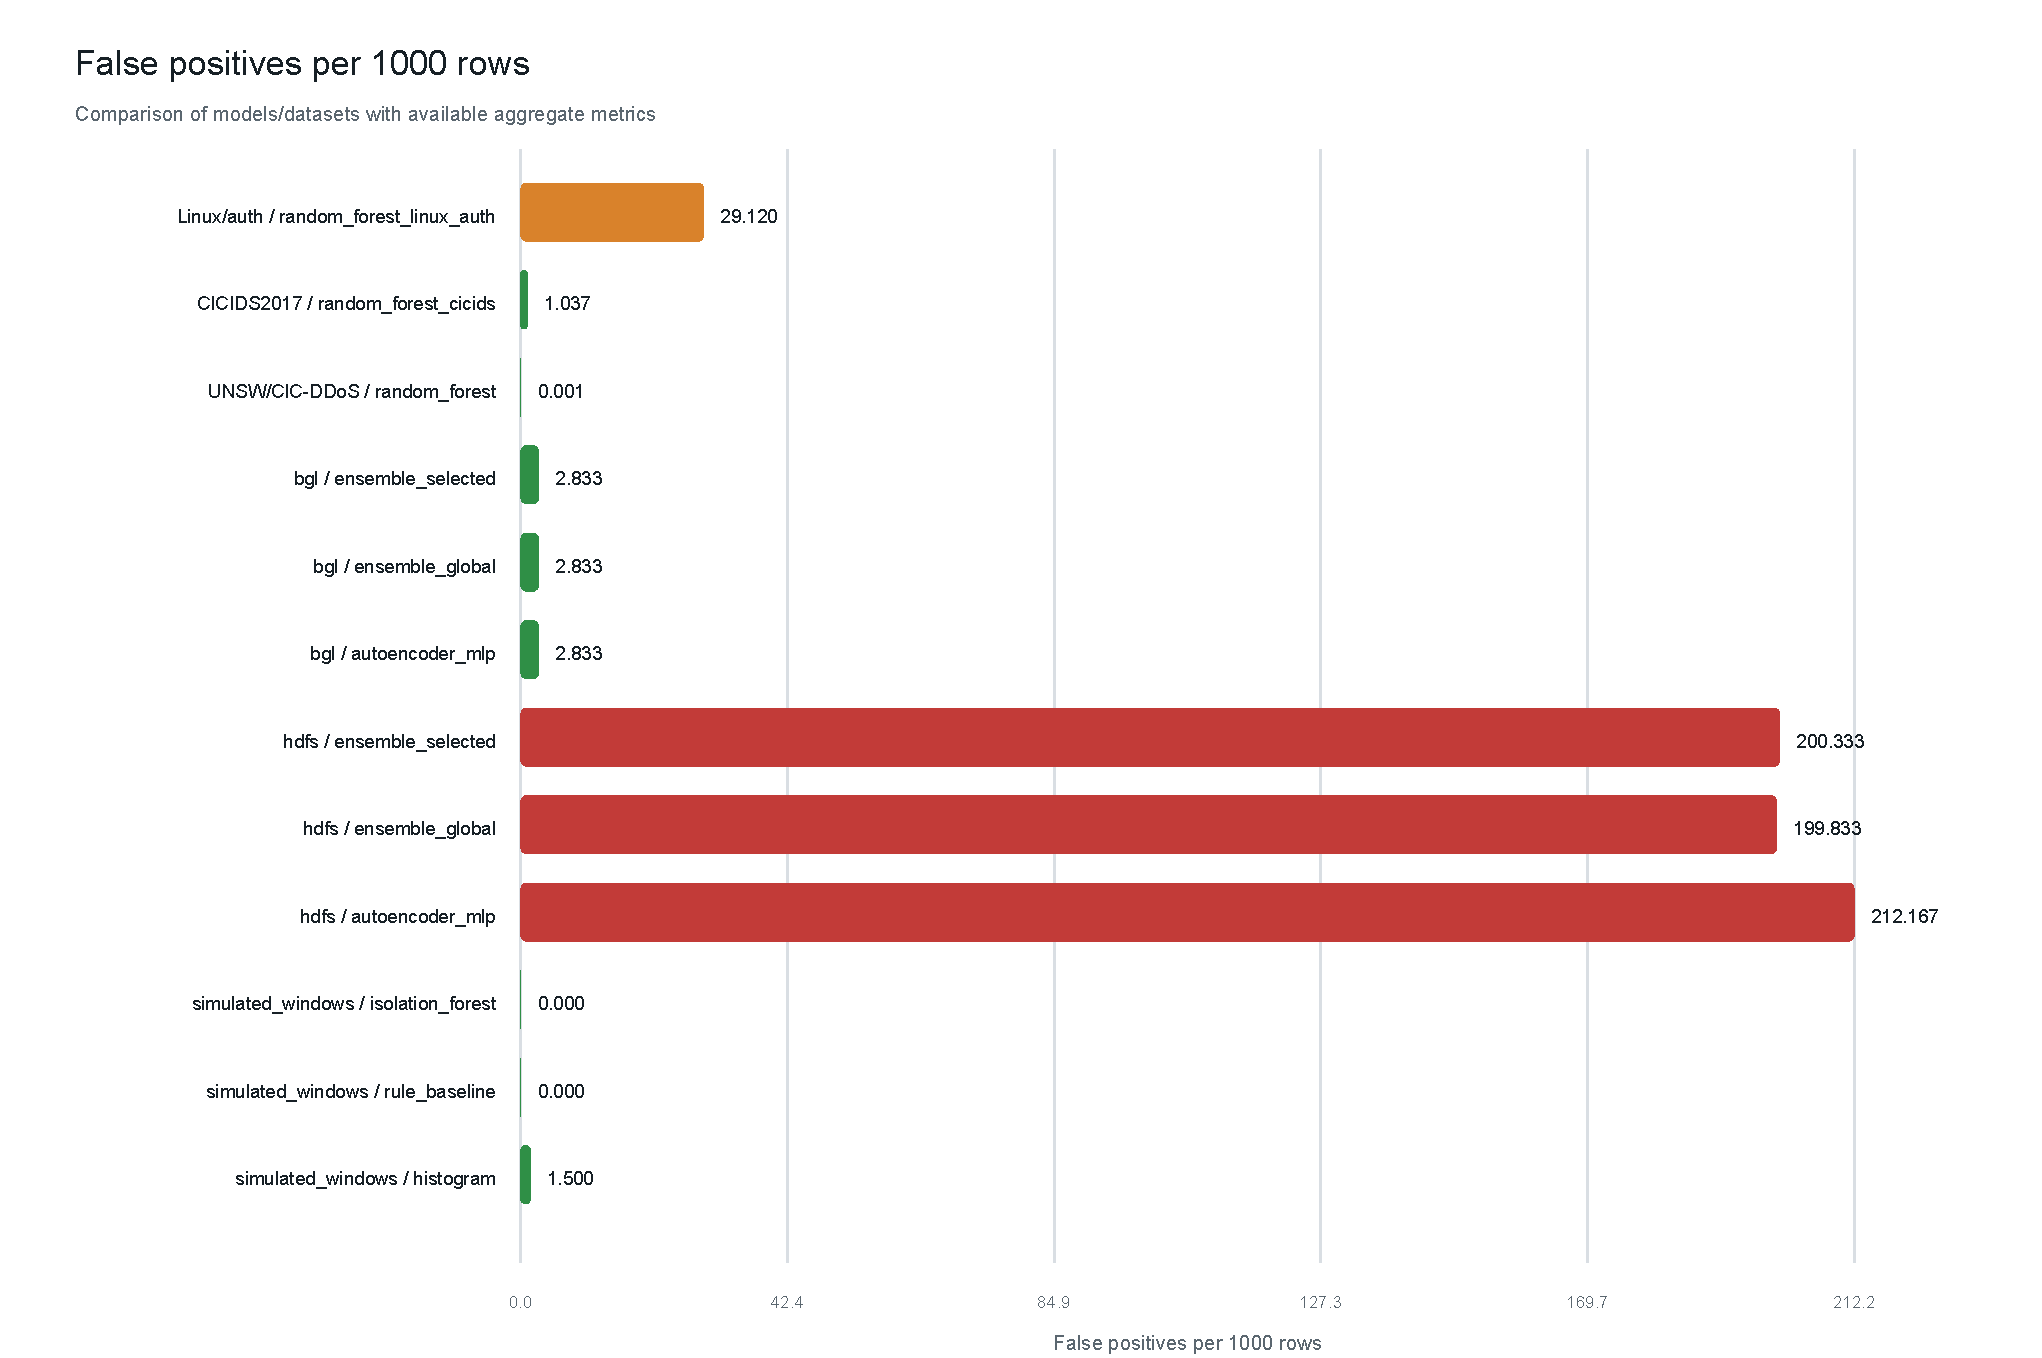
\includegraphics[width=\linewidth]{figures/fig_false_positive_rates.pdf}
    \caption{False positive rates observed by log family and model. HDFS highlights the limitation of lightweight row-level features for sequence-oriented distributed-system logs.}
    \label{fig:falsepos}
\end{figure}

\subsection{Robustness and Workflow Performance}
The parser and normalizer were tested on Apache, CEF/LEEF, CloudTrail, Linux/auth and incomplete logs. The objective is not to claim full universal parsing, but to verify that unexpected or corrupted lines are preserved as unknown records without interrupting the workflow.

\begin{figure}[t]
    \centering
    
\includegraphics[width=\linewidth]{figures/fig_robustness_multiformat.pdf}
    \caption{Robustness check on multi-format inputs. Unknown or incomplete entries are preserved instead of breaking the pipeline.}
    \label{fig:robustness}
\end{figure}

The FastAPI quasi-real-time workflow was executed for 10 cycles with 8,537 lines per cycle on 4 June 2026. All 10 cycles completed successfully. Within this workflow, routing averaged 0.2466 seconds, while detection averaged 5.0801 seconds and correlation 0.7815 seconds. Routing itself is based on a bounded sample and a fixed number of family scores; its approximate cost is $O(k \times c \times s)$, where $k$ is the number of families, $c$ the inspected columns and $s$ the sampled rows. A direct profiling run on 8,537 normalized Windows events shows that the router accounts for 0.9\% of the measured routing-detection-correlation time, while model inference accounts for 91.3\% and correlation for 7.7\% (Table~\ref{tab:timing_profile}). These measurements are included only to show that auditable routing is not the dominant bottleneck in the local prototype. A complete resource, stress and scalability analysis is intentionally reserved for an operational companion study.

\begin{table}[t]
\caption{Direct timing profile on 8,537 normalized Windows events}
\label{tab:timing_profile}
\centering
\scriptsize
\begin{tabular}{l r r}
\toprule
\textbf{Step} & \textbf{Seconds} & \textbf{Share} \\
\midrule
Router & 0.0449 & 0.9\% \\
Detector & 4.3460 & 91.3\% \\
Correlator & 0.3678 & 7.7\% \\
\bottomrule
\end{tabular}
\end{table}

\section{General Discussion and Limitations}
\subsection{Comparison with Standard Tools}
A common reviewer objection is that ELK, OSSEC, Wazuh or fail2ban already process logs. This paper does not dispute their operational value. ELK-like stacks mainly provide ingestion, indexing, search, storage and visualization. Wazuh and OSSEC provide mature HIDS/SIEM functions based on agents, decoders and rules. fail2ban provides direct operational reaction to repeated authentication failures. \logminer{} is different in scope: it focuses on analytical specialization, dynamic model selection by log family, unification of supervised and non-supervised outputs as anomaly candidates, and correlation into analyst-readable incidents.

\begin{table}[t]
\caption{Qualitative positioning against standard tools}
\label{tab:tools}
\centering
\scriptsize
\begin{tabularx}{\linewidth}{p{1.6cm}X X X}
\toprule
\textbf{Criterion} & \textbf{Logminer} & \textbf{fail2ban} & \textbf{OSSEC/Wazuh} \\
\midrule
Detection & Statistical/AI anomalies and contextual correlation & Rules on authentication failures and IP banning & Rules, decoding and HIDS/SIEM alerts \\
Sources & Windows, Linux, Wazuh, HDFS, BGL, network, cloud & Mainly exposed services and auth logs & Broad source coverage through agents and decoders \\
Adaptation & Multi-model routing by family & Manual filters and thresholds & Rules, lists and SOC configuration \\
Positioning & Lightweight analytical complement & Immediate operational protection & Mature production HIDS/SIEM base \\
\bottomrule
\end{tabularx}
\end{table}

\subsection{Scope and Limitations}
Table~\ref{tab:limits} states the defensible scope of the prototype. This scope is necessary to avoid overclaiming.

Consistent with the project steering document, the intended deployment context is a lightweight analysis workstation, laboratory environment, small or medium organization, or intermediate gateway that complements existing log-management tools. \logminer{} is not presented as a large-enterprise SIEM replacement, a full SOC ingestion platform, or a detector to be installed heavily on every endpoint.

The high HDFS false positive rate is an important example of this scope boundary. It does not invalidate the family-aware architecture, but it shows that sequential distributed-system logs require a different downstream detector family than lightweight row-level scoring. Because \logminer{} separates normalization, routing and detection, a future HDFS/BGL branch can route normalized events toward a Drain-like template parser followed by sequence-aware detection, while simpler tabular branches such as Linux/auth, CICIDS2017 and UNSW/CIC-DDoS continue to use lighter supervised models. This modularity is central to the proposed architecture: heavier algorithms can be attached only where the log family requires them.

\begin{table}[t]
\caption{Scope and limitations of the prototype}
\label{tab:limits}
\centering
\scriptsize
\begin{tabularx}{\linewidth}{p{2.1cm}X}
\toprule
\textbf{Point} & \textbf{Defensible position} \\
\midrule
Software agents & Specialized cooperating software modules plus bounded supervisor control, not fully cognitive autonomous agents \\
Distribution & Logical and local service distribution; multi-machine deployment remains future work \\
Adaptive AI & Policy-based routing and workflow parameter adaptation, not continuous self-learning or optimized planning \\
Real time & Local quasi-real-time workflow, not strict industrial SOC real time \\
Asynchronism & Redis Streams queue and workers exist as an implementation path; measured queue scaling, back-pressure, retries and dead-letter handling are reserved for the operational article \\
Deployment & Current prototype targets an analysis workstation, laboratory setup, small/medium organization or intermediate gateway, not a large-enterprise SOC platform or a heavy detector installed on every endpoint \\
Tool comparison & Analytical complement to Wazuh/fail2ban/OSSEC, not replacement \\
Unsupervised results & Anomaly candidates, not confirmed intrusions \\
\bottomrule
\end{tabularx}
\end{table}

\subsection{Threats to Validity}
The main internal validity threat is that results combine multiple datasets, feature representations and model families. The controlled ablation mitigates this risk, but also shows that routing alone is not always superior under a common minimal feature space. The operational ablation evaluates routing, specialized feature spaces and specialized detectors together; it does not isolate the independent contribution of each factor. Therefore, the claim is limited to controlled specialization and feature/model compatibility, not universal dominance over monolithic classifiers. A stricter factorial design would require at least three independent axes: router choice, feature representation and detector family.

Statistical validity is limited because repeated-seed confidence intervals and broad routing-weight sensitivity sweeps are not yet reported. The current router constants are auditable policy parameters, but they are not calibrated probabilities; the added $\pm10\%$ replay only covers the five SupervisorAgent sources and should be interpreted as a local stability check. Dataset validity is also limited: very high F1 scores on network datasets require careful interpretation because class imbalance, duplicate flows, temporal splitting and train-test leakage can distort intrusion-detection benchmarks. HDFS demonstrates an explicit negative boundary of the current lightweight row-level representation and should be compared against sequence-aware parsers and detectors before any stronger claim is made for distributed-system logs. Model-persistence validity is also relevant: the June 2026 benchmark environment loaded several scikit-learn model artifacts trained under earlier library versions, which generated compatibility warnings. The results are still useful as local prototype measurements. The repository now includes a Dockerfile and a pinned \texttt{requirements-container.txt} file to document the runtime environment, but exact external replication of the reported F1 scores still requires retraining or republishing model artifacts under that pinned environment. Long-running stress, resource and supervisor-degradation results are not used as central evidence in this article.

External validity is limited by the selected datasets and local execution environment. Operational validity is limited because non-supervised anomalies require analyst confirmation, correlation quality is not yet evaluated against analyst-labeled incidents, and a real SOC deployment would require stronger ingestion guarantees, access control, retention policies, back-pressure handling, response workflows and stress tests over longer campaigns.

\section{Conclusion and Future Work}
This paper presented \logminer, a lightweight auditable family-aware routing architecture for heterogeneous log anomaly detection. Its main contribution is a specialization layer that makes model selection explicit, preserves routing reasons and fallback behavior, and connects common normalization with compatible family-specific detectors and interpretable correlation. Results across Windows, Wazuh, Linux/auth, HDFS, BGL, CICIDS2017 and UNSW/CIC-DDoS support the feasibility of the approach on a local infrastructure.

The ablation study refines the contribution: the family-aware strategy should be understood as controlled specialization rather than a guarantee of better F1 on every source. Further work includes a factorial ablation separating routing, features and model choice; stronger template-based parsing; routing HDFS/BGL-style logs toward a Drain-like semantic parsing agent followed by temporal or LSTM-style sequence detection; multi-machine deployment; active learning from analyst decisions; richer incident explanations; and integration with mature SIEM/HIDS platforms. Detailed supervisor stability, stress, resource and scalability campaigns are reserved for a separate operational study.

\section*{Declaration of Generative AI and AI-Assisted Technologies}
The authors used AI-assisted writing tools to improve language clarity, structure and readability during manuscript preparation. The authors reviewed, edited and validated the technical content and take full responsibility for the final manuscript.

\balance
\begin{thebibliography}{00}
\bibitem{denning1987intrusion} D. E. Denning, ``An intrusion-detection model,'' \emph{IEEE Transactions on Software Engineering}, vol. SE-13, no. 2, pp. 222--232, 1987, \doiurl{10.1109/TSE.1987.232894}. Available: \url{https://www.cs.colostate.edu/~cs656/reading/ieee-se-13-2.pdf}.
\bibitem{axelsson2000intrusion} S. Axelsson, ``Intrusion detection systems: A survey and taxonomy,'' Technical Report, Chalmers University of Technology, 2000. Available: \url{https://www.cse.msu.edu/~cse960/Papers/security/axelsson00intrusion.pdf}.
\bibitem{sommer2010outside} R. Sommer and V. Paxson, ``Outside the closed world: On using machine learning for network intrusion detection,'' in \emph{IEEE Symposium on Security and Privacy}, 2010, pp. 305--316, \doiurl{10.1109/SP.2010.25}.
\bibitem{chandola2009anomaly} V. Chandola, A. Banerjee, and V. Kumar, ``Anomaly detection: A survey,'' \emph{ACM Computing Surveys}, vol. 41, no. 3, pp. 1--58, 2009, \doiurl{10.1145/1541880.1541882}.
\bibitem{buczak2016survey} A. L. Buczak and E. Guven, ``A survey of data mining and machine learning methods for cyber security intrusion detection,'' \emph{IEEE Communications Surveys and Tutorials}, vol. 18, no. 2, pp. 1153--1176, 2016, \doiurl{10.1109/COMST.2015.2494502}.
\bibitem{khraisat2019survey} A. Khraisat, I. Gondal, P. Vamplew, and J. Kamruzzaman, ``Survey of intrusion detection systems: Techniques, datasets and challenges,'' \emph{Cybersecurity}, vol. 2, no. 20, 2019, \doiurl{10.1186/s42400-019-0038-7}.
\bibitem{he2016drain} P. He, J. Zhu, Z. Zheng, and M. R. Lyu, ``Drain: An online log parsing approach with fixed depth tree,'' in \emph{IEEE International Conference on Web Services}, 2017, pp. 33--40, \doiurl{10.1109/ICWS.2017.13}. Available: \url{https://jiemingzhu.github.io/pub/pjhe_icws2017.pdf}.
\bibitem{zhu2023loghub} J. Zhu, S. He, P. He, J. Liu, and M. R. Lyu, ``Loghub: A large collection of system log datasets for AI-driven log analytics,'' in \emph{IEEE International Symposium on Software Reliability Engineering}, 2023, pp. 355--366, \doiurl{10.1109/ISSRE59848.2023.00071}. Available: \url{https://github.com/logpai/loghub}.
\bibitem{du2017deeplog} M. Du, F. Li, G. Zheng, and V. Srikumar, ``DeepLog: Anomaly detection and diagnosis from system logs through deep learning,'' in \emph{ACM CCS}, 2017, pp. 1285--1298, \doiurl{10.1145/3133956.3134015}.
\bibitem{meng2019loganomaly} W. Meng, Y. Liu, Y. Zhu, S. Zhang, D. Pei, Y. Liu, Y. Chen, R. Zhang, S. Tao, P. Sun, and R. Zhou, ``LogAnomaly: Unsupervised detection of sequential and quantitative anomalies in unstructured logs,'' in \emph{International Joint Conference on Artificial Intelligence}, 2019, pp. 4739--4745, \doiurl{10.24963/ijcai.2019/658}.
\bibitem{zhang2019logrobust} X. Zhang, Y. Xu, Q. Lin, B. Qiao, H. Zhang, Y. Dang, C. Xie, X. Yang, Q. Cheng, Z. Li, J. Chen, X. He, R. Yao, J.-G. Lou, M. Chintalapati, F. Shen, and D. Zhang, ``Robust log-based anomaly detection on unstable log data,'' in \emph{ACM Joint Meeting on European Software Engineering Conference and Symposium on the Foundations of Software Engineering}, 2019, pp. 807--817, \doiurl{10.1145/3338906.3338931}.
\bibitem{guo2021logbert} H. Guo, S. Yuan, and X. Wu, ``LogBERT: Log anomaly detection via BERT,'' in \emph{International Joint Conference on Neural Networks}, 2021, pp. 1--8, \doiurl{10.1109/IJCNN52387.2021.9534113}.
\bibitem{balasubramaniyan1998aafid} J. S. Balasubramaniyan, J. O. Garcia-Fernandez, D. Isacoff, E. Spafford, and D. Zamboni, ``An architecture for intrusion detection using autonomous agents,'' in \emph{Annual Computer Security Applications Conference}, 1998, pp. 13--24. Available: \url{https://zzamboni.org/files/pubs/aafid-acsac98.pdf}.
\bibitem{jacobs1991moe} R. A. Jacobs, M. I. Jordan, S. J. Nowlan, and G. E. Hinton, ``Adaptive mixtures of local experts,'' \emph{Neural Computation}, vol. 3, no. 1, pp. 79--87, 1991, \doiurl{10.1162/neco.1991.3.1.79}.
\bibitem{mirsky2018kitsune} Y. Mirsky, T. Doitshman, Y. Elovici, and A. Shabtai, ``Kitsune: An ensemble of autoencoders for online network intrusion detection,'' in \emph{Network and Distributed System Security Symposium}, 2018, \doiurl{10.14722/ndss.2018.23204}.
\bibitem{nist80092} National Institute of Standards and Technology, ``Guide to computer security log management,'' NIST Special Publication 800-92, 2006, \doiurl{10.6028/NIST.SP.800-92}.
\bibitem{rfc5424} R. Gerhards, ``The Syslog Protocol,'' RFC 5424, 2009, \doiurl{10.17487/RFC5424}.
\end{thebibliography}

\end{document}
